\chapter{Negapedia}\label{negapedia}
    \textquote{The development of Wikipedia articles is not always a peaceful and collaborative process} --- as \citeauthor{Sumi} pointed out in \cite{Sumi}.  Extreme cases of disagreement over an article content --- where editors repeatedly override each other's contribution --- is called an edit war: it is usually very unconstructive.
    
    Wikipedia's edit wars --- and, more generally, Wikipedia's edit histories --- provide very important insights into societal controversies \cite{Borra}: articles often inherit the conflicts of the external world they seek to document. However, users can't easily understand how the information contained in each Wikipedia page evolves over time: they are only exposed to a single possible representation of a topic, which is shaped by editors with different opinions and biased towards some commercial interests.
    
    With the aim of showing to the general public this \textquote{dark} side of Wikipedia and its hidden information, in \citeyear{MarchioriNegapedia} \citeauthor{MarchioriNegapedia} briefly introduced \emph{Negapedia} \cite{MarchioriNegapedia} (the project has then been more extensively discussed in \cite{MarchioriBattle}). Negapedia is a website that measures the contrasts hidden behind every Wikipedia page: \blockquote[\url{http://en.negapedia.org/about/}]{Like every social interaction, the creation of articles in Wikipedia is subject to a balancing between “positive” and “negative” forces, where people add or delete information in reaction to different impulses. In fact, information is not just made of facts but also of needs, contrapositions, biases, interests. These aspects trigger epic battles in many parts of Wikipedia, battles that evolve over time and mirror our society, with its multitude of opinions and consequent clashes.}
    \section{Negativity behind Wikipedia articles}
        Though there are many ways in which negativity behind each Wikipedia article can be measured and displayed, only two measures have been selected: \emph{conflict} and \emph{polemic} \cite{MarchioriNegapedia}. \citeauthor{MarchioriNegapedia} justify this choice by saying that usability must be kept in mind and that it is usually difficult to understand an issue when one has too much information about it --- the so-called information overload.
        \subsection{Conflict}
            Edit wars can have different forms. Negapedia focuses on reverts --- i. e. actions that undo or negate the effects of one or more edits, which result in the page being restored to an old version. For example, different editors may revert each other's edits repeatedly.
            
            Conflict somehow quantifies the negativity behind each Wikipedia article: it is defined as the number of users --- which may be bots --- that have been involved in a revert \cite{MarchioriBattle} (instead of taking into account the actual number of reverts, Negapedia focuses on the social conflict that lies underneath a page \cite{MarchioriNegapedia}). Therefore, the higher the conflict behind a page, the more stable the content is. On the other hand, a low level of conflict corresponds to a page whose content is mostly stable.
        \subsection{Polemic}
            Though conflict measures the absolute quantity of negativity, it does not say anything about the relative negativity within the social community of a page. Indeed, a page with many contributors is likely to have a higher conflict than a page with only very few contributors.
            
            Polemic --- the second measure used by Negapedia to study the negativity behind Wikipedia articles --- solves these issues by taking into account \textquote{quality} rather than quantity.
            
            The metric used to measure polemic is not the simple ratio of editors involved in an edit war. Instead, it is a product of two terms \cite{MarchioriNegapedia}:
            \begin{itemize}
                \item The ratio between conflict and popularity (number of authors of a page) measures how much the conflict behind a page is important.
                \item The ratio between the overall number of articles and the number of articles having both a bigger conflict and a lower popularity measures the rarity of the specific instance.
            \end{itemize}
            Formally, polemic is defined as follows:
            \[polemic = \frac{conflict}{popularity} \cdot log\left(\frac{\sharp articles}{\sharp articles \quad \mid \quad \ge conflict\, \land\, \le popularity}\right)\]
        \subsection{Displaying negativity}
            Negapedia is meant to be easy to use: therefore, only selected information is showed to the user \cite{MarchioriNegapedia}:
            \begin{itemize}
                \item The system shows how conflict and polemic change over time for every Wikipedia article. See figure \ref{conflict_polemic} for an example. 
                \begin{figure}
                    \centering
                    \includegraphics[width=\textwidth]{images/conflict-polemic.png}
                    \caption{Conflict and polemic over time for the Harry Potter page of the English edition of Wikipedia (as of May 2019).}
                    \label{conflict_polemic}
                \end{figure}
                \item Negapedia keeps track of the top 10 most negative pages over time and categories\footnote{\url{http://en.negapedia.org/about/top-tens}.}. Top ten lists are a compact and quick way to summarize and display information about the most negative pages of Wikipedia.
                \item \textquote{Awards}\footnote{\url{http://en.negapedia.org/about/awards}.} are assigned to very negative Wikipedia pages. An award is basically granted every time a page is included in a top ten list. See figure \ref{awards} for an example.
                \begin{figure}
                    \centering
                    \includegraphics[width=0.7\textwidth]{images/awards.png}
                    \caption{Awards for conflict --- as of May 2019 --- given to the Garry Kasparov page of the English edition of Wikipedia.}
                    \label{awards}
                \end{figure}
                \item \textquote{Social jumps}\footnote{\url{http://en.negapedia.org/about/social-jumps}.} provide an alternate way to navigate Wikipeia pages: they connect pages that are socially related, in the sense that they have a number of editors in common.
            \end{itemize}
    \section{Assigning Wikipedia articles to macro categories}\label{negapedia_categories}
        Negapedia divides Wikipedia articles into \emph{macro categories} in order to make it easier for the user to see separately the negative side of various aspects of our society. The algorithm behind articles categorization relies on the graph structure of Wikipedia --- formed by a high number of hyperlinks --- and it propagates information using the concept of absorbing Markov chain.
        \subsection{Macro categories}
            Negapedia divides Wikipedia articles into macro categories that roughly correspond to the main Wikipedia portals\footnote{A portal supplement the encyclopedia by providing a variety of sample content of subtopics and by improving navigability within a vast amount of knowledge. Basically, it is an enhanced \textquote{main page} for a broad subject.}. Though originally \citeauthor{MarchioriNegapedia} have chosen to divide Wikipedia articles into 10 categories \cite{MarchioriNegapedia}, the current version of Negapedia --- as of May 2019 --- uses an additional one\footnote{\url{http://en.negapedia.org/categories/}.}:
            \begin{multicols}{2}
                \begin{itemize}
                    \item Culture, arts and entertainment
                    \item Geography and places
                    \item Health and fitness
                    \item History and events
                    \item Mathematics and logic
                    \item Nature and physical sciences
                    \item People and self
                    \item Philosophy and thinking
                    \item Religion and belief systems
                    \item Society and social sciences
                    \item Technology and applied sciences
                \end{itemize}
            \end{multicols}
        \subsection{Algorithm}\label{negapedia_algorithm}
            The category of each Wikipedia article is automatically computed by an algorithm originally developed in \cite{Bonetti}, which works on an \textquote{extended semantic graph}. Such a graph can be built as follows:
            \begin{enumerate}
                \item First, the semantic graph\footnote{A graph whose vertices represent concepts and whose edges represent semantic relations between concepts.} of Wikipedia articles is created. Specifically, the algorithm builds a directed graph (the so-called \emph{Wikigraph} \cite{Buriol}) where Wikipedia articles --- i.e., vertices --- are interconnected by hyperlinks --- i.e., edges. The structure of this graph is similar to that of Web, but more densely linked \cite{Kamps}.
                \item Then, the algorithm uses Wikipedia categories to build a taxonomy-like structure called \emph{Wikipedia Category Graph} (WCG) \cite{Zesch}. It should be noticed, though, that Wikipedia does not strictly enforce a taxonomic category structure: cycles and disconnected components in this graph are possible (see section \ref{wikipedia:categories} for more details).
                \item Since each Wikipedia article can link to an arbitrary number of Wikipedia categories, it is possible to merge these two graphs, obtaining the \textquote{extended semantic graph}.
            \end{enumerate}
            \begin{figure}
    \centering
    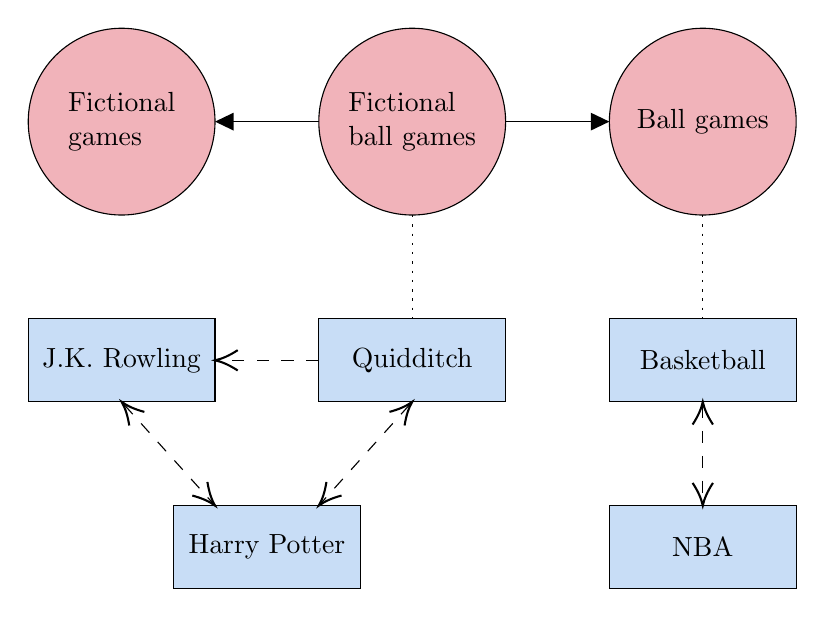
\begin{tikzpicture}[x=0.75pt,y=0.75pt,yscale=-1,xscale=1]
        %Shape: Circle [id:dp8115219034229394] 
        \draw  [fill={rgb, 255:red, 208; green, 2; blue, 27 }  ,fill opacity=0.3 ] (10,55) .. controls (10,30.15) and (30.15,10) .. (55,10) .. controls (79.85,10) and (100,30.15) .. (100,55) .. controls (100,79.85) and (79.85,100) .. (55,100) .. controls (30.15,100) and (10,79.85) .. (10,55) -- cycle ;
        %Shape: Circle [id:dp8163711353091557] 
        \draw  [fill={rgb, 255:red, 208; green, 2; blue, 27 }  ,fill opacity=0.3 ] (150,55) .. controls (150,30.15) and (170.15,10) .. (195,10) .. controls (219.85,10) and (240,30.15) .. (240,55) .. controls (240,79.85) and (219.85,100) .. (195,100) .. controls (170.15,100) and (150,79.85) .. (150,55) -- cycle ;
        %Shape: Circle [id:dp9514147881884653] 
        \draw  [fill={rgb, 255:red, 208; green, 2; blue, 27 }  ,fill opacity=0.3 ] (290,55) .. controls (290,30.15) and (310.15,10) .. (335,10) .. controls (359.85,10) and (380,30.15) .. (380,55) .. controls (380,79.85) and (359.85,100) .. (335,100) .. controls (310.15,100) and (290,79.85) .. (290,55) -- cycle ;
        %Straight Lines [id:da26929607637664343] 
        \draw    (150,55) -- (102,55) ;
        \draw [shift={(100,55)}, rotate = 360] [fill={rgb, 255:red, 0; green, 0; blue, 0 }  ][line width=0.75]  [draw opacity=0] (8.93,-4.29) -- (0,0) -- (8.93,4.29) -- cycle    ;
        
        %Straight Lines [id:da55975302746763] 
        \draw    (240,55) -- (288,55) ;
        \draw [shift={(290,55)}, rotate = 180] [fill={rgb, 255:red, 0; green, 0; blue, 0 }  ][line width=0.75]  [draw opacity=0] (8.93,-4.29) -- (0,0) -- (8.93,4.29) -- cycle    ;
        
        %Shape: Rectangle [id:dp5695294519694281] 
        \draw  [fill={rgb, 255:red, 74; green, 144; blue, 226 }  ,fill opacity=0.3 ] (150,150) -- (240,150) -- (240,190) -- (150,190) -- cycle ;
        %Shape: Rectangle [id:dp9459907669998763] 
        \draw  [fill={rgb, 255:red, 74; green, 144; blue, 226 }  ,fill opacity=0.3 ] (10,150) -- (100,150) -- (100,190) -- (10,190) -- cycle ;
        %Shape: Rectangle [id:dp9118915462525985] 
        \draw  [fill={rgb, 255:red, 74; green, 144; blue, 226 }  ,fill opacity=0.3 ] (80,240) -- (170,240) -- (170,280) -- (80,280) -- cycle ;
        %Shape: Rectangle [id:dp706551589936829] 
        \draw  [fill={rgb, 255:red, 74; green, 144; blue, 226 }  ,fill opacity=0.3 ] (290,150) -- (380,150) -- (380,190) -- (290,190) -- cycle ;
        %Shape: Rectangle [id:dp23087103101225726] 
        \draw  [fill={rgb, 255:red, 74; green, 144; blue, 226 }  ,fill opacity=0.3 ] (290,240) -- (380,240) -- (380,280) -- (290,280) -- cycle ;
        %Straight Lines [id:da05502265811536389] 
        \draw  [dash pattern={on 4.5pt off 4.5pt}]  (150,170) -- (102,170) ;
        \draw [shift={(100,170)}, rotate = 360] [color={rgb, 255:red, 0; green, 0; blue, 0 }  ][line width=0.75]    (10.93,-4.9) .. controls (6.95,-2.3) and (3.31,-0.67) .. (0,0) .. controls (3.31,0.67) and (6.95,2.3) .. (10.93,4.9)   ;
        
        %Straight Lines [id:da5354993058131741] 
        \draw  [dash pattern={on 4.5pt off 4.5pt}]  (193.66,191.49) -- (151.34,238.51) ;
        \draw [shift={(150,240)}, rotate = 311.99] [color={rgb, 255:red, 0; green, 0; blue, 0 }  ][line width=0.75]    (10.93,-4.9) .. controls (6.95,-2.3) and (3.31,-0.67) .. (0,0) .. controls (3.31,0.67) and (6.95,2.3) .. (10.93,4.9)   ;
        \draw [shift={(195,190)}, rotate = 131.99] [color={rgb, 255:red, 0; green, 0; blue, 0 }  ][line width=0.75]    (10.93,-4.9) .. controls (6.95,-2.3) and (3.31,-0.67) .. (0,0) .. controls (3.31,0.67) and (6.95,2.3) .. (10.93,4.9)   ;
        %Straight Lines [id:da11087403714951327] 
        \draw  [dash pattern={on 4.5pt off 4.5pt}]  (56.34,191.49) -- (98.66,238.51) ;
        \draw [shift={(100,240)}, rotate = 228.01] [color={rgb, 255:red, 0; green, 0; blue, 0 }  ][line width=0.75]    (10.93,-4.9) .. controls (6.95,-2.3) and (3.31,-0.67) .. (0,0) .. controls (3.31,0.67) and (6.95,2.3) .. (10.93,4.9)   ;
        \draw [shift={(55,190)}, rotate = 48.01] [color={rgb, 255:red, 0; green, 0; blue, 0 }  ][line width=0.75]    (10.93,-4.9) .. controls (6.95,-2.3) and (3.31,-0.67) .. (0,0) .. controls (3.31,0.67) and (6.95,2.3) .. (10.93,4.9)   ;
        %Straight Lines [id:da7909762012355506] 
        \draw  [dash pattern={on 4.5pt off 4.5pt}]  (335,192) -- (335,238) ;
        \draw [shift={(335,240)}, rotate = 270] [color={rgb, 255:red, 0; green, 0; blue, 0 }  ][line width=0.75]    (10.93,-4.9) .. controls (6.95,-2.3) and (3.31,-0.67) .. (0,0) .. controls (3.31,0.67) and (6.95,2.3) .. (10.93,4.9)   ;
        \draw [shift={(335,190)}, rotate = 90] [color={rgb, 255:red, 0; green, 0; blue, 0 }  ][line width=0.75]    (10.93,-4.9) .. controls (6.95,-2.3) and (3.31,-0.67) .. (0,0) .. controls (3.31,0.67) and (6.95,2.3) .. (10.93,4.9)   ;
        %Straight Lines [id:da5382710413033004] 
        \draw  [dash pattern={on 0.84pt off 2.51pt}]  (195,100) -- (195,150) ;
        
        %Straight Lines [id:da6347712182350267] 
        \draw  [dash pattern={on 0.84pt off 2.51pt}]  (335,100) -- (335,150) ;
        
        % Text Node
        \draw (55,55) node  [align=left] {Fictional\\games};
        % Text Node
        \draw (195,55) node  [align=left] {Fictional\\ball games};
        % Text Node
        \draw (335,55) node  [align=left] {Ball games};
        % Text Node
        \draw (195,170) node  [align=left] {Quidditch};
        % Text Node
        \draw (335,260) node  [align=left] {NBA};
        % Text Node
        \draw (125,260) node  [align=left] {Harry Potter};
        % Text Node
        \draw (55,170) node  [align=left] {J.K. Rowling};
        % Text Node
        \draw (335,170) node  [align=left] {Basketball};
    \end{tikzpicture}
    \caption{Example of an extended semantic graph, as presented in \cite{Bonetti}. Blue nodes represent the semantic graph of Wikipedia articles --- the so-called \textquote{Wikigraph} \cite{Buriol} --- and red nodes represent the taxonomy-like structure of Wikipedia categories --- the so-called Wikipedia Category Graph (WCG) \cite{Zesch}. These two graphs can be merged thanks to the fact that each Wikipedia article can be linked to a number of categories. Edges drawn in dissimilar styles model different semantic relations between nodes.}
    \label{extended_semantic_graph}
\end{figure}
            An example of the extended semantic graph can be seen in figure \ref{extended_semantic_graph}.
            
            The macro categories --- or topics, as they are called in \cite{Bonetti} --- are chosen among the categories: the approach presented by \citeauthor{Bonetti} requires that macro categories to be vertices of the extended semantic graph.
            
            Once the graph has been built and the topics chosen, the algorithm models the process of assigning Wikipedia articles to macro categories as an absorbing Markov chain. Specifically, nodes that represent categories or articles are modeled as transient states, and nodes that represent topics are modeled as absorbing states. Moreover, a probability is assigned to each edge of the graph using experimental values.
            
            To formally define the transient matrix \(P\) of the absorbing Markov chain, \citeauthor{Bonetti} introduced the concepts of \emph{distance} and \emph{weight}. Let \(G\left(V,E\right)\) be the extended semantic graph, and let \(\left(i,j\right)\) be the edge that links nodes \(i\) and \(j\). Also, let \(c \in \left[0,1\right]\) be a constant and \(A \subset V\) the set of transient states. Then:
            \begin{description}
                \item[distance] \(d\left(v\right)\), with \(v \in V\), is the length of the shortest from \(v\) to a topic. Only edges whose source or target is a category can be used.
                \item[weight] \(
                    w\left(i,j\right) =
                    \begin{cases}
                        c & \text{if \(j \in A\)} \\
                        \frac{1}{1+10\cdot\left(d\left(j\right)-d\left(i\right)+1\right)} & \text{otherwise}
                    \end{cases}
                \)
            \end{description}
            
            Using these functions, the \(p_{ij}\) element of the transient matrix can be formally defined as:
            \[p_{ij} = \frac{w\left(i,j\right)}{\sum_{v \in V}w\left(i,v\right)}\]
            
            An optimal value of the constant \(c\) has been found performing a number of experiments. For the Italian edition of Wikipedia, experiments have clearly shown that \(c\) should be in the range \(\left[\frac{1}{30},\frac{1}{90}\right]\). However, this constant has to be tuned for each Wikipedia edition, and this turned out to be one of the main problems of the approach presented in \cite{Bonetti} by \citeauthor{Bonetti}.